
\documentclass[aspectratio=169]{beamer}

% activate me to make slides with no animation
%\documentclass[handout]{beamer}


\usepackage[warn]{mathtext}
\usepackage[T2A]{fontenc}
\usepackage[utf8]{inputenc}
\usepackage[english,russian]{babel}

\usepackage{amssymb}
\usepackage{amsmath}
\usepackage{multirow}
\usepackage{graphicx}
\usepackage{verbatim}
\usepackage{comment} 
\usepackage{minted}

\usepackage{listings}
\lstset{language=Java,
                basicstyle=\footnotesize\ttfamily,
                keywordstyle=\footnotesize\color{blue}\ttfamily,
}


%%%%%%%%%%%%%%%%%%%%%%%%%%%%%%%%%  fix-lstlinebgrd.tex 
\makeatletter
\let\old@lstKV@SwitchCases\lstKV@SwitchCases
\def\lstKV@SwitchCases#1#2#3{}
\makeatother
\usepackage{lstlinebgrd}
\makeatletter
\let\lstKV@SwitchCases\old@lstKV@SwitchCases
        
\lst@Key{numbers}{none}{%
    \def\lst@PlaceNumber{\lst@linebgrd}%
    \lstKV@SwitchCases{#1}%
    {none:\\%
     left:\def\lst@PlaceNumber{\llap{\normalfont
                \lst@numberstyle{\thelstnumber}\kern\lst@numbersep}\lst@linebgrd}\\%
     right:\def\lst@PlaceNumber{\rlap{\normalfont
                \kern\linewidth \kern\lst@numbersep
                \lst@numberstyle{\thelstnumber}}\lst@linebgrd}%
    }{\PackageError{Listings}{Numbers #1 unknown}\@ehc}}
\makeatother
%%%%%%%%%%%%%%%%%%%%%%%%%%%%%%%%%


%%%%%%%%%%%%%%%%%%%%%%%%%%%%%%%%%  bListHL
\makeatletter
%%%%%%%%%%%%%%%%%%%%%%%%%%%%%%%%%%%%%%%%%%%%%%%%%%%%%%%%%%%%%%%%%%%%%%%%%%%%%%
%
% \btIfInRange{number}{range list}{TRUE}{FALSE}
%
% Test in int number <number> is element of a (comma separated) list of ranges
% (such as: {1,3-5,7,10-12,14}) and processes <TRUE> or <FALSE> respectively

\newcount\bt@rangea
\newcount\bt@rangeb

\newcommand\btIfInRange[2]{%
    \global\let\bt@inrange\@secondoftwo%
    \edef\bt@rangelist{#2}%
    \foreach \range in \bt@rangelist {%
        \afterassignment\bt@getrangeb%
        \bt@rangea=0\range\relax%
        \pgfmathtruncatemacro\result{ ( #1 >= \bt@rangea) && (#1 <= \bt@rangeb) }%
        \ifnum\result=1\relax%
            \breakforeach%
            \global\let\bt@inrange\@firstoftwo%
        \fi%
    }%
    \bt@inrange%
}
\newcommand\bt@getrangeb{%
    \@ifnextchar\relax%
        {\bt@rangeb=\bt@rangea}%
        {\@getrangeb}%
}
\def\@getrangeb-#1\relax{%
    \ifx\relax#1\relax%
        \bt@rangeb=100000%   \maxdimen is too large for pgfmath
    \else%
        \bt@rangeb=#1\relax%
    \fi%
}
%%%%%%%%%%%%%%%%%%%%%%%%%%%%%%%%%%%%%%%%%%%%%%%%%%%%%%%%%%%%%%%%%%%%%%%%%%%%%%
%
% \btLstHL<overlay spec>{range list}
%
% TODO BUG: \btLstHL commands can not yet be accumulated if more than one overlay spec match.
%
\newcommand<>{\btLstHL}[1]{%
\only#2{\btIfInRange{\value{lstnumber}}{#1}{\color{yellow}\def\lst@linebgrdcmd{\color@block}}{\def\lst@linebgrdcmd####1####2####3{}}}%
}%

\newcommand<>{\btLstHLG}[1]{%
\only#2{\btIfInRange{\value{lstnumber}}{#1}{\color{green}\def\lst@linebgrdcmd{\color@block}}{\def\lst@linebgrdcmd####1####2####3{}}}%
}%
\makeatother
%%%%%%%%%%%%%%%%%%%%%%%%%%%%%%%%%



\usetheme{CambridgeUS}

% tikz
\usepackage{pgf}
\usepackage{tikz}
\usepackage{tikz-qtree}
\usetikzlibrary{arrows, automata, fit, shapes, shapes.multipart, trees, positioning}

\usepackage{array}
\usepackage{cancel}
\usepackage{hyperref}
\usepackage[normalem]{ulem}


\newtheorem{homeworkmail}[theorem]{Homework, mail}

\newcommand{\showTOC}{
    \begin{frame}[noframenumbering,plain]
        \frametitle{Lecture plan}
        \tableofcontents[currentsection]
    \end{frame}
}

\newcommand{\showTOCSub}{
    \begin{frame}[noframenumbering,plain]
        \frametitle{Lecture plan}
        \tableofcontents[currentsubsection]
    \end{frame}
}


\newcommand{\questiontime}[1]{
    \begin{frame}[noframenumbering,plain]
        \frametitle{Question time}

        Question: #1

        \begin{center}
            
\includegraphics[width=0.4\textwidth]{../../common/pics/coins.png}
        \end{center}

        
    \end{frame}
}



\newcommand{\orgNum}{0}
\newcommand{\orgTopic}{org meeting}
\newcommand{\orgKey}{syllabus, contacts}

\newcommand{\introNum}{1}
\newcommand{\introTopic}{introduction to multithreading}
\newcommand{\introKey}{concurrency, parallelism, agents, threads, scheduler, Amdahl's law, race condition, deadlock, wait-for graph}

\newcommand{\basicNum}{2}
\newcommand{\basicTopic}{basic concepts}
\newcommand{\basicKey}{mutex, acquisition order, reentrancy, fairness, data locking, code locking, signalling, condition variable, lost signal, spurious wakeup}

\newcommand{\syncPrimitivesNum}{3}
\newcommand{\syncPrimitivesTopic}{advanced synchronization primitives}
\newcommand{\syncPrimitivesKey}{monitor, latch, barrier, thundering herd, semaphore, read-write lock, thread pool, executor, producer-consumer, fork-join, load balancing}

\newcommand{\patternsNum}{4}
\newcommand{\patternsTopic}{advanced synchronization concepts}
\newcommand{\patternsKey}{interruption, cancellation, partitioning, privatization, replication, thread-local, ownership}

\newcommand{\extraBasicsNum}{5}
\newcommand{\extraBasicsTopic}{additional topics of practical concurrency}
\newcommand{\extraBasicsKey}{documenting protocols and classes, checking concurrent invariants, stress testing, execution trace analysis, estimating required testing effort, static and dynamic checks, scheduling randomization, model checking}

\newcommand{\foundationsNum}{6}
\newcommand{\foundationsTopic}{theoretical foundations of concurrency}
\newcommand{\foundationsKey}{timeline, partial order, sequential consistency, linearizability, quiscent consistency, correctness, liveness, safety, atomicity}

\newcommand{\foundationsPlusNum}{7}
\newcommand{\foundationsPlusTopic}{progress guarantees, concurrent operations hierarchy, consensus number}
\newcommand{\foundationsPlusKey}{obstruction-free, lock-free, wait-free, safe register, regular register, atomic register, consensus number, register snapshots}

\newcommand{\atomicsNum}{8}
\newcommand{\atomicsTopic}{introduction to atomics}
\newcommand{\atomicsKey}{compare-and-swap, fetch-and-add, spinning, lock-free stack, taxonomy of queues, ABA problem}

\newcommand{\cacheCoherencyNum}{9}
\newcommand{\cacheCoherencyTopic}{cache coherency}
\newcommand{\cacheCoherencyKey}{cache memory hierarchy, cache coherency protocol. store-buffer, load-buffer, invalidate-queue, memory barrier, hardware memory model, weak memory model, litmus tests}

\newcommand{\langMMNum}{10}
\newcommand{\langMMTopic}{language memory model}
\newcommand{\langMMKey}{motivation, approaches, comparison of existing solutions}

\newcommand{\advancedConcurrencyNum}{11}
\newcommand{\advancedConcurrencyTopic}{advanced concurrency}
\newcommand{\advancedConcurrencyKey}{CLH/MCS queue/lock, backoff policies revisited, notify-as-ready, RAT optimization, single LIFO cell optimization, work distribution, work stealing, taxonomy of parallel problems}

\newcommand{\userSpaceThreadingNum}{12}
\newcommand{\userSpaceThreadingTopic}{user-space threading}
\newcommand{\userSpaceThreadingKey}{berkley socket, blocking and non-blocking IO, callback-hell, async-await, continuation-passing-style, fibers/coroutines/green threads, stackful vs stackless}


\newcommand{\designNum}{13}
\newcommand{\designTopic}{designing concurrent systems}
\newcommand{\designKey}{park/unpark, synchronizer, futex/wait-on-address, plan9 approach, race-finders, ForkJoinPool/CoroutineCarriers/UIthread, observability, structured concurrency}

\newcommand{\frameworksAndDistributedNum}{14}
\newcommand{\frameworksAndDistributedTopic}{multi-agent systems}
\newcommand{\frameworksAndDistributedKey}{auto-parallelization languages and frameworks, semi-automatic synchronization, distributed systems, consensus protocols}


\title[]{Lecture \introNum: \introTopic}
\subtitle[]{\introKey}
\author[]{Alexander Filatov\\ filatovaur@gmail.com}

\date{}


\newcommand{\taskExceptions}{1.1}
\newcommand{\taskAmdhal}{1.2}
\newcommand{\taskEmpire}{1.3}
\newcommand{\taskJstack}{1.4}

\begin{document}

\begin{frame}
  \titlepage
  \url{https://github.com/Svazars/parallel-programming/blob/main/slides/pdf/l1.pdf}
\end{frame}

\begin{frame}{Lecture plan}
\tableofcontents
\end{frame}


\begin{section}{Motivation}

\begin{frame}[fragile]{Motivation}
\framesubtitle{Moore's law}

{\tiny\url{https://en.wikipedia.org/wiki/Moore%27s_law#/media/File:Moore's_Law_Transistor_Count_1970-2020.png}}

\begin{center}
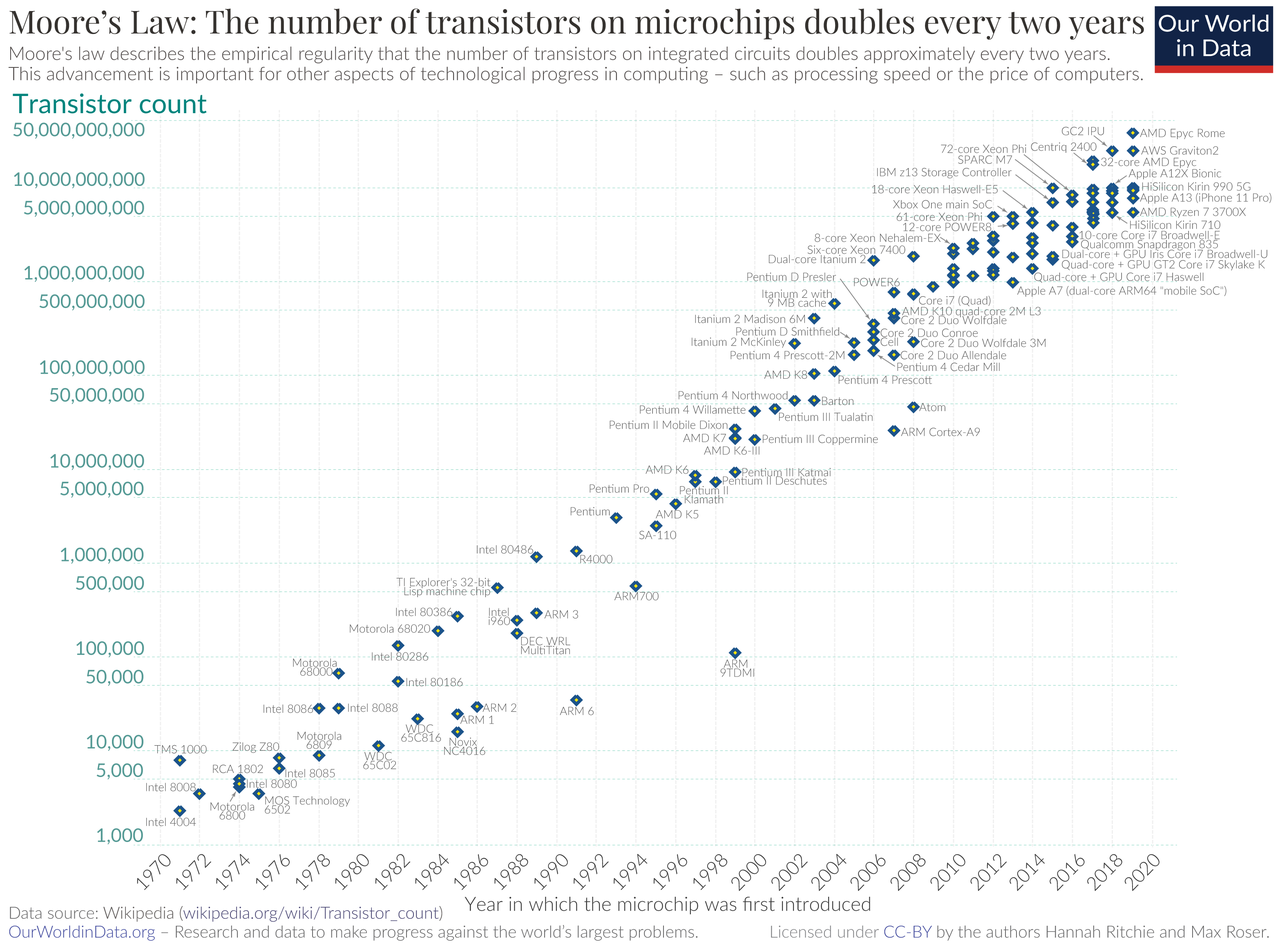
\includegraphics[width=0.5\textwidth]{./pics/transistor_count.png}
\end{center}

\end{frame}


\begin{frame}[fragile]{Motivation}
\framesubtitle{Clock frequency}

{\tiny\url{http://cpudb.stanford.edu/visualize/clock_frequency.html}}

\begin{center}
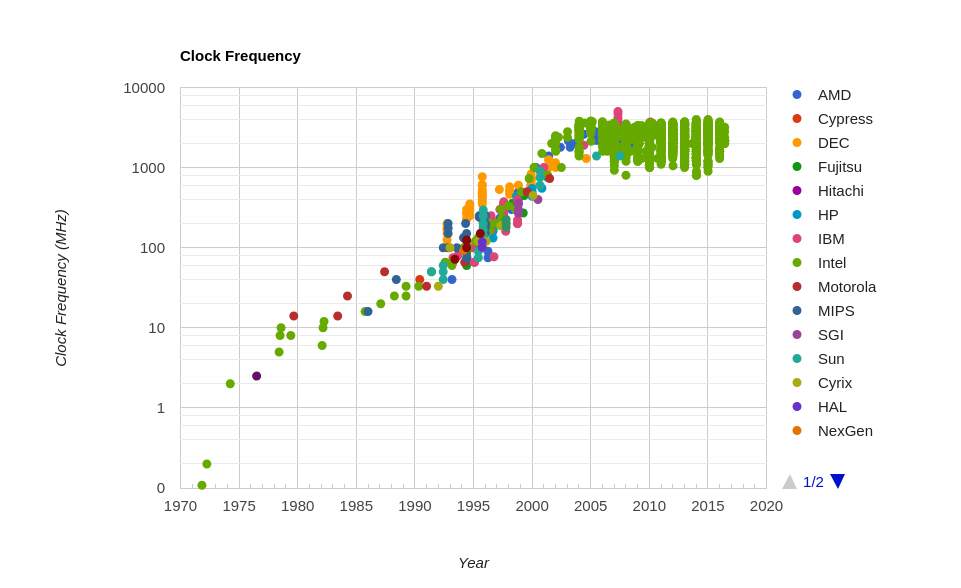
\includegraphics[width=0.6\textwidth]{./pics/clock_freq.png}
\end{center}

\end{frame}

\questiontime{Where are all these transistors?}


\begin{frame}[fragile]{Motivation}
\framesubtitle{Core per CPU}

{\tiny\url{https://www.reddit.com/r/Amd/comments/6cu5ss/highest_amount_of_cores_per_cpu_amd_vs_intel_year}}

\begin{center}
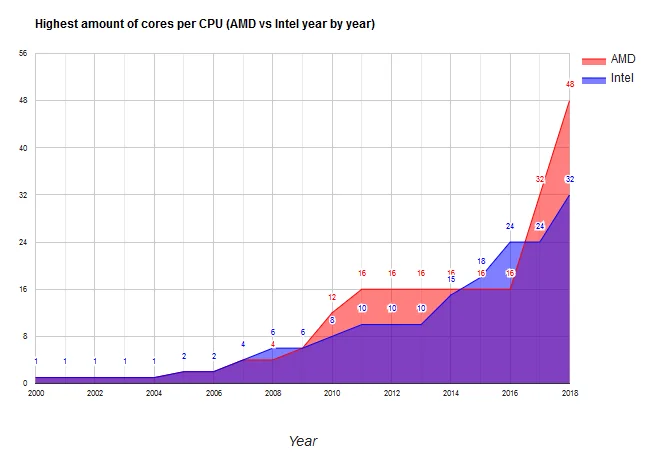
\includegraphics[width=0.5\textwidth]{./pics/core_per_cpu.png}
\end{center}

\end{frame}


\begin{frame}{Motivation}
\framesubtitle{Multi-agent systems}

{\tiny\url{https://sea.mastercard.com/en-region-sea/business/merchants/start-accepting/payment-process.html}}

\begin{center}
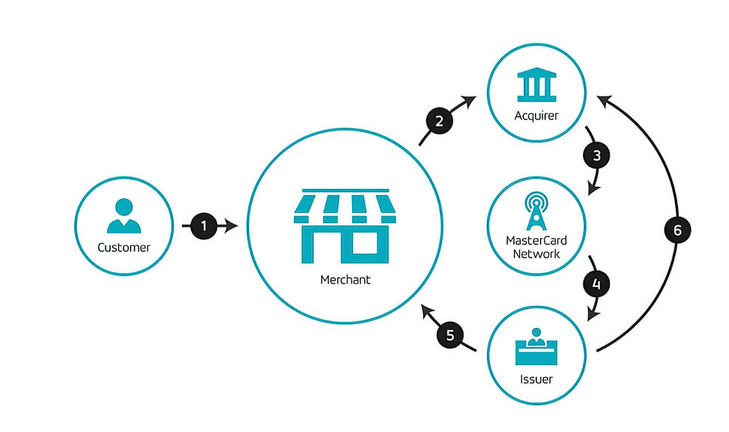
\includegraphics[width=0.5\textwidth]{./pics/mastercard.png}
\end{center}

\end{frame}


\begin{frame}{Motivation}
\framesubtitle{Multi-agent systems}

{\tiny\url{https://en.wikipedia.org/wiki/Apache_Kafka#/media/File:Overview_of_Apache_Kafka.svg}}

\begin{center}
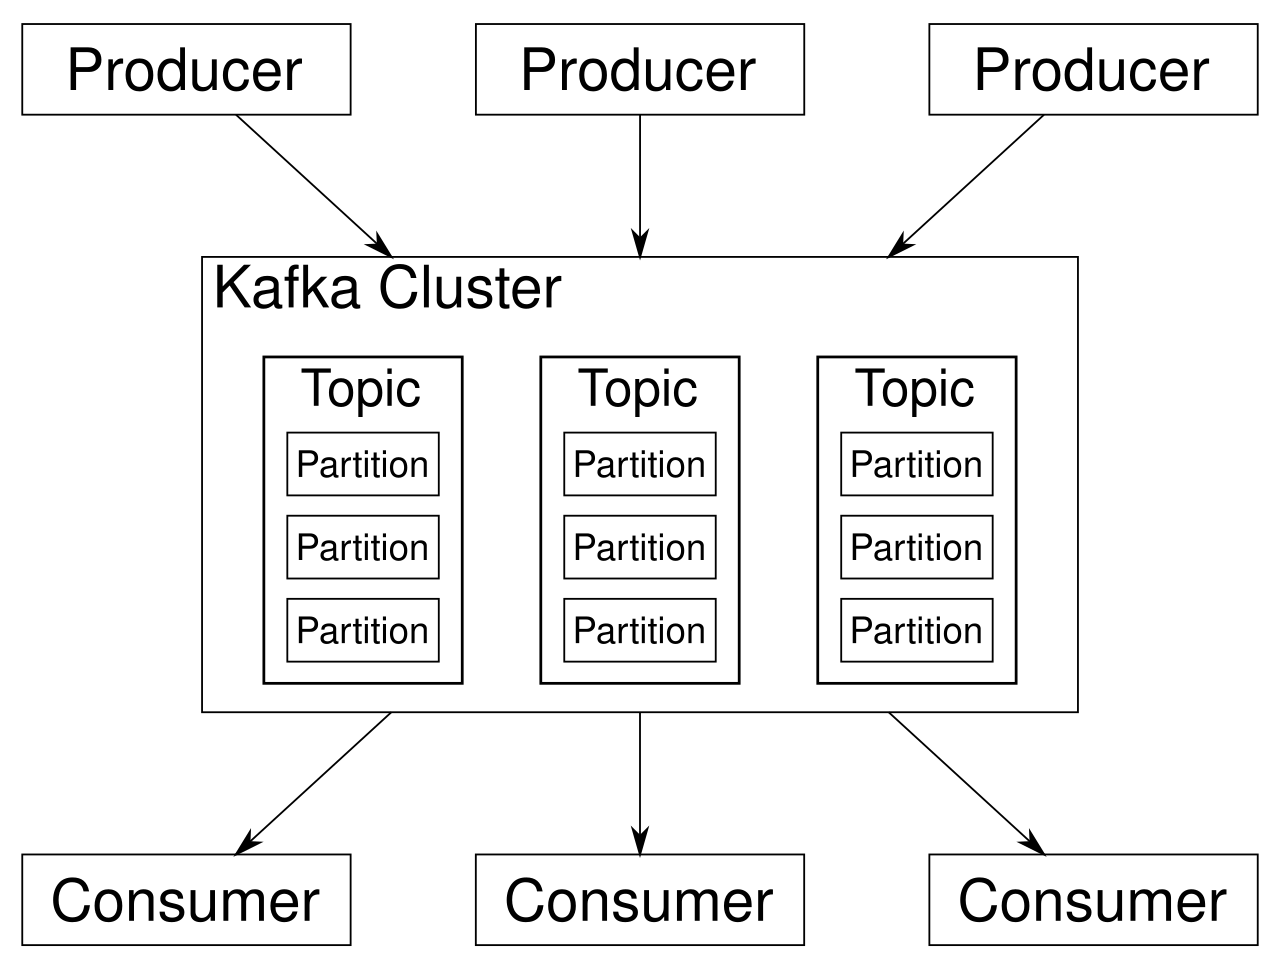
\includegraphics[width=0.5\textwidth]{./pics/kafka.png}
\end{center}

\end{frame}


\begin{frame}{Motivation}
\framesubtitle{Multi-agent systems}

{\tiny\url{https://spark.apache.org/docs/latest/cluster-overview.html}}

\begin{center}
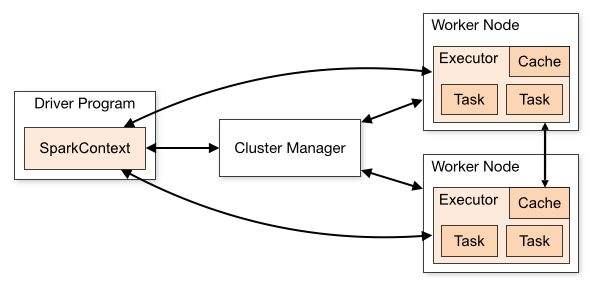
\includegraphics[width=0.5\textwidth]{./pics/spark.png}
\end{center}

\end{frame}


\begin{frame}{Motivation}
\framesubtitle{Multi-agent systems}

{\tiny\url{https://events19.linuxfoundation.org/wp-content/uploads/2018/07/dbueso-oss-japan19.pdf}}

\begin{center}
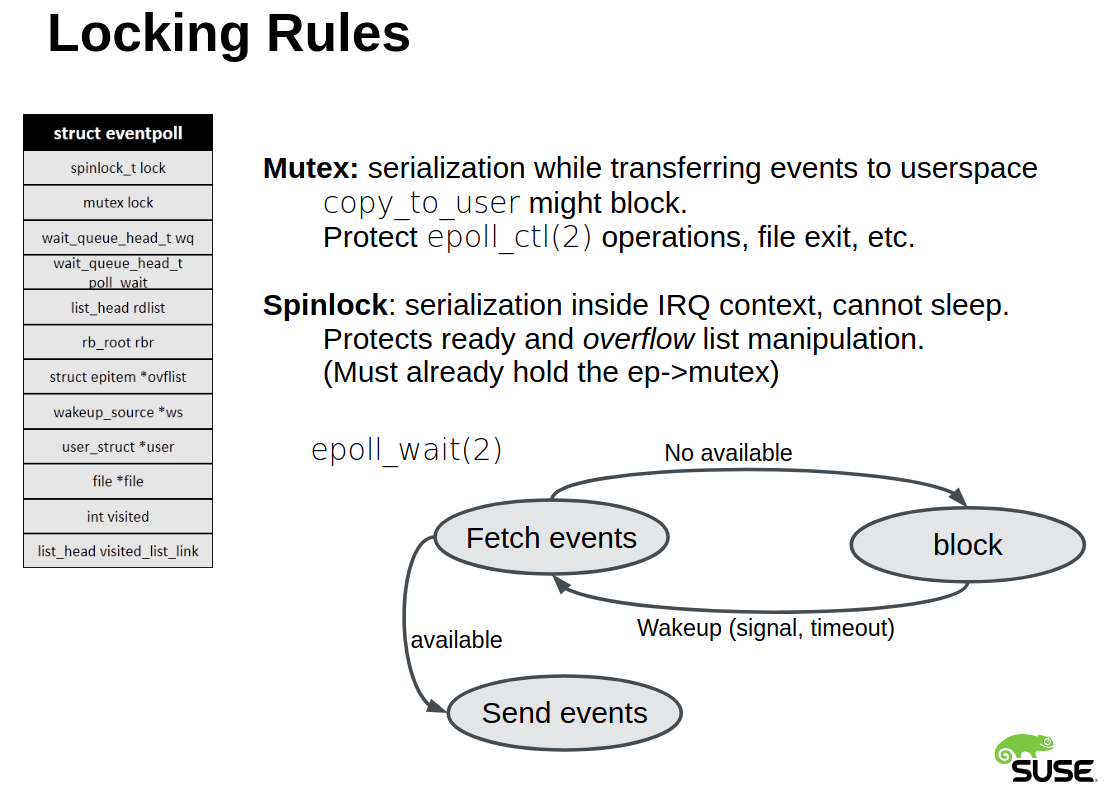
\includegraphics[width=0.5\textwidth]{./pics/epoll_something.png}
\end{center}
\end{frame}


\begin{frame}{Common problems}

\begin{itemize}
    \item Many \textbf{independent} parts
    \item Different \textbf{speed}
    \item Need to \textbf{communicate} with each other
    \item Need to \textbf{coordinate} execution
    \item May \textbf{fail} spuriously
\end{itemize}


%человечество использовало независимо существующие, но взаимодействующие между собой сущности с очень давних времен. В компьютерах просто таких сущностей очень много и взаимодействуют они с безумной частотой. Приходится натравливать другие компьютеры чтобы справляться (картинка битыв работов)
\end{frame}


\begin{frame}{Agents}

This course is about \textbf{communicating agents}. We will see
\begin{itemize}
    \item Alice \& Bob
    \item Processes in operating system
    \item Threads in operating system
    \item Separate computers that use networking to pass messages
    \item ...
\end{itemize}

Agents will try to:
\begin{itemize}
    \item Decide who is in charge
    \item Pass data without corruption
    \item Coordinate execution of several steps in complicated task
    \item Find out how many agents take part in the communication  
    \item ...
\end{itemize}

\end{frame}

\begin{frame}{Different worlds}

There are a lot of basic concepts behind the communication of independent agents.

But worlds are \textit{different}:
\begin{itemize}
    \item timings
    \begin{itemize}
        \item minutes (conversation)
        \item seconds (networking)
        \item milliseconds (shared memory)
        \item nanoseconds (CPU)
    \end{itemize}
    \item delivery 
    \begin{itemize}
        \item possible distortion (misunderstanding)
        \item possible loss (UDP packet)
        \item visibility issue (not-yet-updated memory cell/stale value in CPU cache)
    \end{itemize}
    \item denial-of-service 
    \begin{itemize}
        \item several people do phone call to the same person
        \item network go offline
        \item shared memory of single process in consistent (yet weakly ordered)
    \end{itemize}
    \item ...
\end{itemize}
\end{frame}


\begin{section}{Concurrency and parallelism}

\showTOC

\questiontime{''concurrency'', ''parallelism'', who could translate both words to Russian?}

\begin{frame}[fragile]{Concurrency vs parallelism}
\framesubtitle{Situations}

Sequential and interruptible = concurrent\footnote{\tiny\url{https://go.dev/talks/2012/waza.slide#12}}

\begin{center}
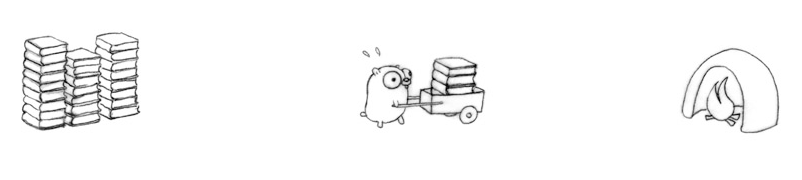
\includegraphics[width=0.5\textwidth]{./pics/gopher_single.png}
\end{center}

\pause

Independent and simultaneous = parallel\footnote<2->{\tiny\url{https://go.dev/talks/2012/waza.slide#15}}

\begin{center}
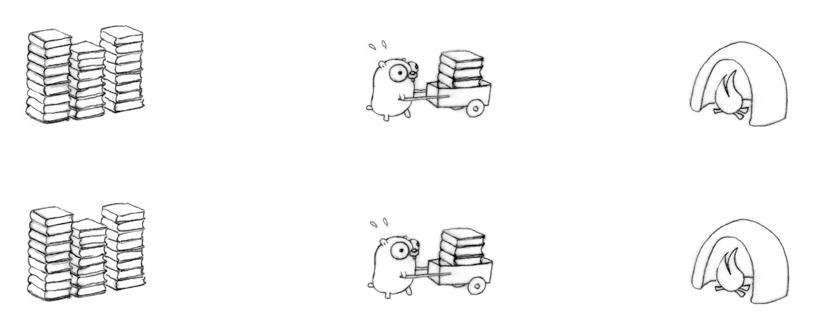
\includegraphics[width=0.4\textwidth]{./pics/gopher_parallel.png}
\end{center}

\end{frame}

\begin{frame}[fragile]{Concurrency vs parallelism}
\framesubtitle{Two sides of the same medal}

Real life is mixed\footnote{\tiny\url{https://go.dev/talks/2012/waza.slide#22}}

\begin{center}
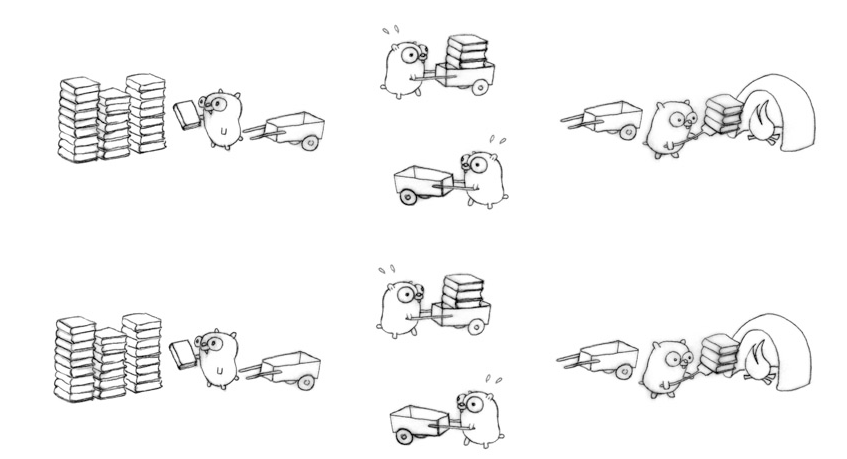
\includegraphics[width=0.5\textwidth]{./pics/gopher_mixed.png}
\end{center}

Fun fact: real people in industry/academia may ''interpret'' parallelism/concurrency in different ways

\end{frame}


\begin{frame}[t]{Concurrency vs parallelism}
\framesubtitle{English}

\begin{itemize}
    \item Parallel
    \item Concurrent
    \item Independent
    \item Simultaneous
    \item At the same time
\end{itemize}

\end{frame}

\questiontime{''Parallel'', ''Concurrent'', ''Independent'', ''Simultaneous'', ''At the same time''. Use one Russian word which would be the best translation for all 5 concepts.}

\begin{frame}[t,noframenumbering]{Concurrency vs parallelism}
\framesubtitle{English}

\begin{itemize}
    \item Parallel
    \item Concurrent
    \item Independent
    \item Simultaneous
    \item At the same time
\end{itemize}

Parallel -- \textit{could} execute simultaneously (independent, applicable to different executors)

Concurrent -- \textit{could} execute interchangeably (interruptible, applicable to the same executor)

Any real-life task combines parallel and concurrent parts\footnote{\tiny\url{https://stackoverflow.com/questions/1050222/what-is-the-difference-between-concurrency-and-parallelism}}.

\end{frame}


\begin{frame}{Concurrency vs parallelism}
\framesubtitle{Time-sharing for users}

Single CPU, many users\footnote{\tiny\url{https://www.geeksforgeeks.org/time-sharing-operating-system/}}

\begin{center}
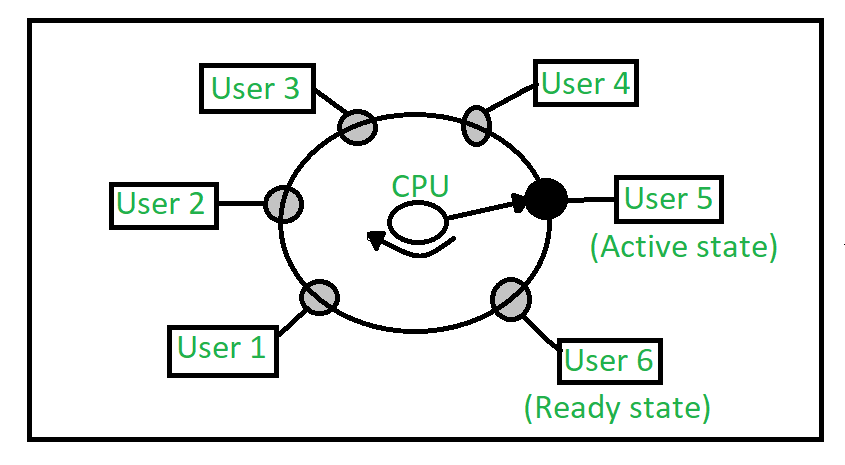
\includegraphics[width=0.6\textwidth]{./pics/time_sharing_one.png}
\end{center}

\end{frame}


\begin{frame}{Concurrency vs parallelism}
\framesubtitle{Time-sharing for tasks}

Single CPU, pre-emptible tasks\footnote{\tiny\url{https://en.wikipedia.org/wiki/CPU_time}}

\begin{center}
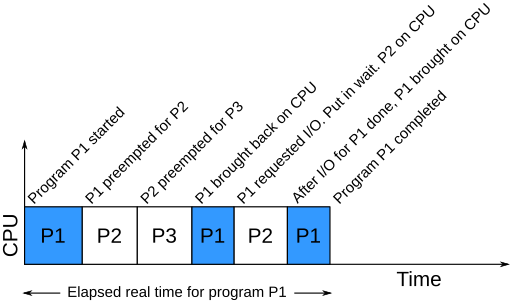
\includegraphics[width=0.6\textwidth]{./pics/time_sharing_two.png}
\end{center}

\end{frame}

\begin{frame}{Concurrency vs parallelism}
\framesubtitle{Time-sharing scheduling strategies}

Round-robin scheduling\footnote{\tiny\url{https://en.wikipedia.org/wiki/Round-robin_scheduling}}

\begin{center}
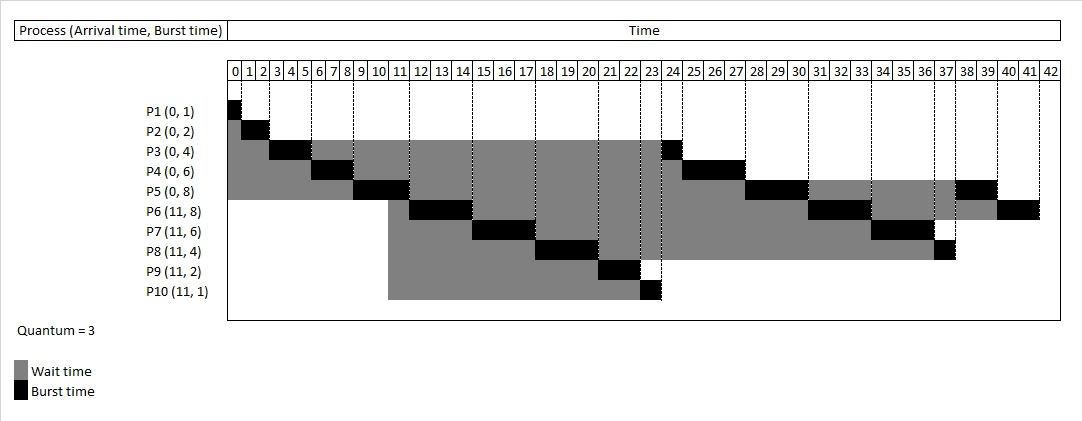
\includegraphics[width=0.8\textwidth]{./pics/round_robin.png}
\end{center}

%Many core, many tasks
%Example with bash, fork, wait and concurrent printing stuff on few-core cpu.

\end{frame}


\begin{frame}{Concurrency vs parallelism}
\framesubtitle{Conclusion}

Concurrency and parallelism are two edges of the same phenomena.

In computer science (and in our course) 
\begin{itemize}
    \item parallelism
    \item concurrency
    \item interruptibility
    \item independence
\end{itemize}

have more formal meaning than in ''usual'' communication. Be aware.

\end{frame}

\begin{section}{Threads and processes}
\showTOC

\questiontime{Difference between ''threads'' and ''processes'' in one word?}

\begin{frame}{Threads vs processes}
\framesubtitle{Blast from the past}

Process\footnote{\tiny\url{https://en.wikipedia.org/wiki/Process_(computing)}}
\begin{itemize}
    \item instance of computer program (program code and other stuff like .data, .rodata, .bss ...)
    \item owns resources (RAM, CPU, network ...) allocated by OS
    \item has logical and physical access permissions (filesystem, user capabilities ...)
    \item described by state (context)    
    \item managed by OS
    \item \textbf{isolated} from other processes (virtual memory, namespaces ...)
\end{itemize}
\end{frame}

\begin{frame}[noframenumbering]{Threads vs processes}
\framesubtitle{Blast from the past}


Thread\footnote{\tiny\url{https://en.wikipedia.org/wiki/Thread_(computing)}}
\begin{itemize}
    \item part of process (executes some code in some context)
    \item owns thread-specific resources (stack, TLS ...)
    \item has specific metadata (priority, TID ...)
    \item described by state (context)
    \item managed by OS scheduler   
    \item \textbf{shares} memory with other threads
\end{itemize}
\end{frame}


\begin{frame}[t]{Threads vs processes}
\framesubtitle{Bird-eye view}

Processes and threads are \textbf{agents}
\begin{itemize}
    \item different speed
    \item could communicate
    \item need coordination
\end{itemize}

\end{frame}

\questiontime{Threads need \textit{more} or \textit{less} coordination compared to processes?}


\begin{frame}[t,noframenumbering]{Threads vs processes}
\framesubtitle{Bird-eye view}

Processes and threads are \textbf{agents}
\begin{itemize}
    \item different speed
    \item could communicate
    \item need coordination
\end{itemize}

\pause
In some sense, threads need \textit{less} coordination (memory is already shared).

\pause
In some sense, threads need \textit{more} coordination (memory is already shared).
\end{frame}


\begin{frame}[fragile]{Threads vs processes}
\framesubtitle{Examples: process}

\begin{tabular}{p{5cm}p{5cm}}

\begin{lstlisting}
echo "Sequential"
wc 50_000_000.txt



real    0m 4,900s
user    0m 4,212s
sys     0m 0,240s
\end{lstlisting}

 & 

\begin{lstlisting}
echo "Parallel"
{ ( head -n 25000000 50_000_000.txt | wc) & }
{ ( tail -n 25000000 50_000_000.txt | wc) & }
wait

real    0m 2,323s
user    0m 4,576s
sys     0m 1,084s
\end{lstlisting}

\end{tabular}

\pause
\begin{itemize}
     \item Create processes
     \item Wait completion
     \item Pass data via pipes, files, advanced IPC
\end{itemize}

\end{frame}

\begin{frame}[fragile]{Threads vs processes}
\framesubtitle{Examples: pthreads\footnote{POSIX threads: \url{https://en.wikipedia.org/wiki/Pthreads}}.}

\textbf{Step 1.} Define and allocate utility struct

\begin{minted}{c}
  struct thread_info {    /* Used as argument to thread_start() */
    pthread_t thread_id;  /* ID returned by pthread_create() */
    int       thread_num; /* Application-defined thread # */
  };

  struct thread_info * tinfo_a = malloc(sizeof(struct thread_info));
  if (tinfo_a == NULL) handle_error("malloc");
\end{minted}
\end{frame}


\begin{frame}[fragile,noframenumbering]{Threads vs processes}
\framesubtitle{Examples: pthreads}

\textbf{Step 2.} Initialize thread attributes
\begin{minted}{c}
  pthread_attr_t attr;
  s = pthread_attr_init(&attr);
  if (s != 0) handle_error("pthread_attr_init");
\end{minted}


\textbf{Step 3.} Define thread body
\begin{minted}{c}
  static void * thread_A_start(void *arg) {
    struct thread_info *tinfo = arg;
    printf("Thread A id = %d: hello world!\n", tinfo->thread_num);
    return NULL;
  }
\end{minted}
\end{frame}

\begin{frame}[fragile,noframenumbering]{Threads vs processes}
\framesubtitle{Examples: pthreads}

\textbf{Step 4.} Initialize utility struct and start new thread
\begin{minted}{c}
  tinfo_a->thread_num = 1;
  s = pthread_create(&(tinfo_a->thread_id), &attr, &thread_A_start, tinfo_a);
  if (s != 0) handle_error("pthread_create");
\end{minted}

\textbf{Step 5.} Join thread
\begin{minted}{c}
  void *res;
  s = pthread_join(tinfo_a->thread_id, &res);
  if (s != 0) handle_error("pthread_join");
  printf("Joined with thread A, result= %p\n", (char *) res);
\end{minted}
\end{frame}

\begin{frame}[fragile,noframenumbering]{Threads vs processes}
\framesubtitle{Examples: pthreads}

\begin{tabular}{p{5cm}p{5cm}}

\begin{minted}{c}
  struct thread_info {
    pthread_t thread_id;
    int       thread_num;
  };
\end{minted}
 & 
\begin{minted}{c}
  static void * thread_A_start(void *arg) {
    struct thread_info *tinfo = arg;
    printf("Thread A id = %d: hello world!\n", 
      tinfo->thread_num);
    return NULL;
  }
\end{minted}
\end{tabular}

\begin{minted}{c}
  // ...
  tinfo_a->thread_num = 1;
  pthread_create(&(tinfo_a->thread_id), &attr, &thread_A_start, tinfo_a);
  pthread_join(tinfo_a->thread_id, &res);
  printf("Joined with thread A, result= %p\n", (char *) res);
\end{minted}

\end{frame}


\begin{frame}[fragile]{Threads vs processes}
\framesubtitle{Examples: Java threads}

\begin{minted}{java}
static class ThreadA extends Thread {
    private int idx;        
    ThreadA(int i) { this.idx = i; }
    @Override
    public void run() {
        System.out.printf("Thread A, idx = %d: hello world\n", this.idx);
    }
}
public static void main(String... args) throws Exception {
    Thread t = new ThreadA(1);
    t.start(); // !!! not t.run !!!
    t.join();
}
\end{minted}
\end{frame}

\questiontime{Why somebody would use Java for parallel programming course, not C or C++?}

\begin{frame}[fragile]{Java threads and exceptions}

Thread \textbf{A} starts thread \textbf{B} and \texttt{join}s. Uncaught exception happens in thread \textbf{B}. 

\begin{itemize}
    \item What happens in thread \textbf{B}?
    \item What happens in thread \textbf{A}?
    \item What if thread \textbf{C} \texttt{join}s thread \textbf{B} \textit{after} exception happened?
    \item What if thread \textbf{D} \texttt{join}s thread \textbf{A}?
\end{itemize}

\pause

\begin{homeworkmail}{Task \taskExceptions}
    Create 3 Java programs for these cases, explain results in several sentences.
}
\end{homeworkmail}

\end{frame}


%\begin{frame}{Threads vs processes}
%\framesubtitle{More serious}
%Строгое определение процесса и потока из Таненбаума.
%Более формальная задача планирования, аливерды в теорию расписаний, пометка про динамическую суть задачи.
%\end{frame}


\begin{frame}{Threads vs processes}
\framesubtitle{Conclusion}

From our course perspective:
\begin{itemize}
    \item processes hold all the context and resources
    \item processes use many different parts of OS
    \item threads use ultra-fast shared memory for communication 
    \item threads are minimal units eligible for OS scheduler
\end{itemize}

Almost all lectures will be about
\begin{itemize}
    \item inter-process multi-threading 
    \item inside high-level programming language
    \item run by multiprocessor hardware with MMU
    \item on non-real-time OS with \only<1>{pre-emptive multitasking}\only<2>{\textbf{pre-emptive multitasking}}    
\end{itemize}
\end{frame}

\begin{section}{Scheduler}
\showTOC

\begin{frame}{Scheduler}
\framesubtitle{Problem overview}

{\tiny\url{https://en.wikipedia.org/wiki/Process_(computing)#/media/File:Concepts-_Program_vs._Process_vs._Thread.jpg}}

\begin{center}
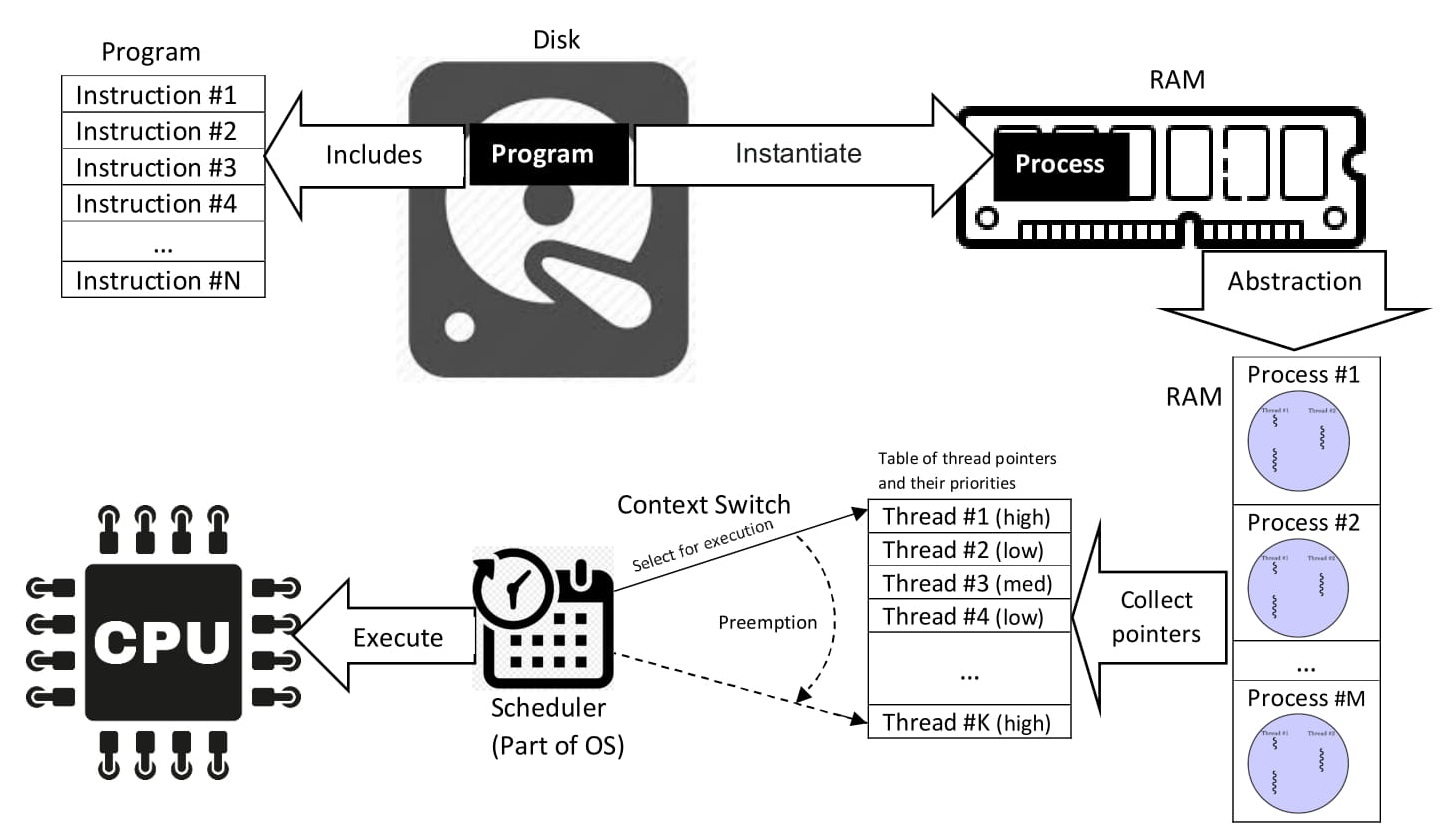
\includegraphics[width=0.6\textwidth]{./pics/full_process_pic.png}
\end{center}


\end{frame}

\begin{frame}[noframenumbering]{Scheduler}
\framesubtitle{Problem overview}

Scheduler -- magic black box
\begin{itemize}
    \item ''knows and owns'' every unit of scheduling (thread)
    \item may pre-empt execution of any unit (save state from CPU to memory) 
    \item may enable execution of any pending unit (load state from memory to CPU)
    \item implements some scheduling policy (round-robin, shortest remaining time ...)
\end{itemize}

\pause

Save state / load state == switch CPU context of execution

\end{frame}

\questiontime{What is context switch on modern OS (e.g. Linux) and modern hardware with MMU (e.g. x86\_64 intel Skylake)?}

\begin{frame}{Scheduler}
\framesubtitle{Context switch}

Do not forget all the important data
\begin{itemize}
    \item registers (general-purpose, floating-point, other)
    \item stack pointer
    \item instruction pointer
    \item segmentation/page tables
    \item translation lookaside buffer flush
    \item ...
\end{itemize}

Requires user-space -> kernel space transition.

\pause
Needs \textit{amortization}.

\pause
Scheduling quantum.

\end{frame}


\begin{frame}{Scheduler}
\framesubtitle{Scheduling quantum}

Quantum may be arbitrary function of \texttt{(current task, other tasks, state of OS)}.

Do not forget about
\begin{itemize}
    \item frequency of context switches
    \item ''price'' of context switch
    \item thread priority
    \item process priority
    \item ''price'' of CPU migration 
    \item occupation of other processors
    \item ...
\end{itemize}

It is hard to trust timings\footnote{\url{https://shipilev.net/blog/2014/nanotrusting-nanotime}}\footnote{\url{https://pzemtsov.github.io/2017/07/23/the-slow-currenttimemillis.html}}.

\end{frame}

\begin{frame}{Scheduler}
\framesubtitle{Pre-emptive and cooperative multitasking}

When to context switch?

\begin{tabular}{p{8cm}p{5cm}}

    Anytime anywhere:
    \begin{itemize}
        \item flexible
        \item easy-to-use model
        \item requires additional care
        \item has counter-examples
        \item relies on heuristics
    \end{itemize}

 &     
    When allowed to:
    \begin{itemize}
        \item fine-grained control
        \item nontrivial behaviour
        \item requires additional care
        \item has counter-examples
        \item relies on heuristics
    \end{itemize}
\end{tabular}

\pause

In real environments it is \textbit{always} a hybrid solution\footnote<2->{The long road to lazy preemption: \url{https://lwn.net/Articles/994322/}}.

\end{frame}

\begin{frame}{Scheduler}
\framesubtitle{Goals}

\begin{itemize}
    \item In theory, there exist a \textit{perfect} schedule
    \item In practice, almost any scheduling problem is NP-complete
    \item In applications, workload is dynamically generated on-the-fly
\end{itemize}

\pause

Realistic goals:
\begin{itemize}
    \item Max \textit{utilization}, not max \textit{efficiency}
    \item Reasonable \textit{latency}
    \item Soft/hard \textit{real-time} constraints
    \item \textit{Energy efficiency}
\end{itemize}
\end{frame}

\questiontime{Describe situation when \textit{max utilization} scheduling contradicts \textit{max efficiency} scheduling}

\begin{section}{Concurrent problems}
\showTOC


\begin{frame}{Concurrent blocks you know so far}

\begin{enumerate}
    \item Create new thread
    \item Modify fields concurrently
    \item Join thread
\end{enumerate}

\pause 
Combining \textbf{1} and \textbf{2}:
\begin{itemize}
    \item Solve ''easy'' parallel problems
    \item Encounter logic errors (race conditions)
    \item Encounter concurrent memory access effects (data races)
\end{itemize}

\pause 
Using \textbf{3}:
\begin{itemize}
    \item Encounter visibility bugs (stale value)
    \item Encounter no-progress blocking (deadlock)
    \item Observe slow-progress issues (priority inversion) 
\end{itemize}

\end{frame}


\begin{subsection}{Embarrassingly parallel problems and Amdahl's law}
\showTOCSub

\begin{frame}{Embarrassingly parallel problems}
\framesubtitle{Introduction}

\begin{itemize}
        \item Embarrassingly parallel
        \item Embarrassingly parallelizable
        \item Perfectly parallel
        \item Delightfully parallel
        \item Pleasingly parallel
\end{itemize}

Key properties:
\begin{itemize}
        \item Granularity
        \item Minimal coordination
\end{itemize}
\end{frame}

\questiontime{Any ideas for embarrassingly parallel problems?}

\begin{frame}{Embarrassingly parallel problems}
\framesubtitle{Examples}

\begin{itemize}
    \item function applied to collection of items (\textit{map})
    \begin{itemize}
        \item ray tracing
        \item word count in independent files
        \item proof-of-work crypto
        \item bioinformatics search (BLAST etc)
        \item Discrete Fourier transform
    \end{itemize}

    \item associative operation applied to large array (order-independent \textit{reduce})
    \begin{itemize}
        \item sum of elements in integer array
        \item word count for all books in e-library    
    \end{itemize}

    \item ...
\end{itemize}
\end{frame}


\begin{frame}[fragile]{Amdahl's law}
\framesubtitle{Key ideas}

Any problem consists of \textit{serial} part and \textit{parallel} part.

Speed-up of parallel part depends on computational resources. Serial part is ''fixed work''.

\begin{itemize}
    \item \textbf{Diminishing Returns}: beyond certain point, adding more processors doesn't significantly increase speedup
    \item \textbf{Limited Speedup}: problem cannot be solved faster than serial part
\end{itemize}

{\tiny\url{https://en.wikipedia.org/wiki/Amdahl%27s_law}}
\begin{center}
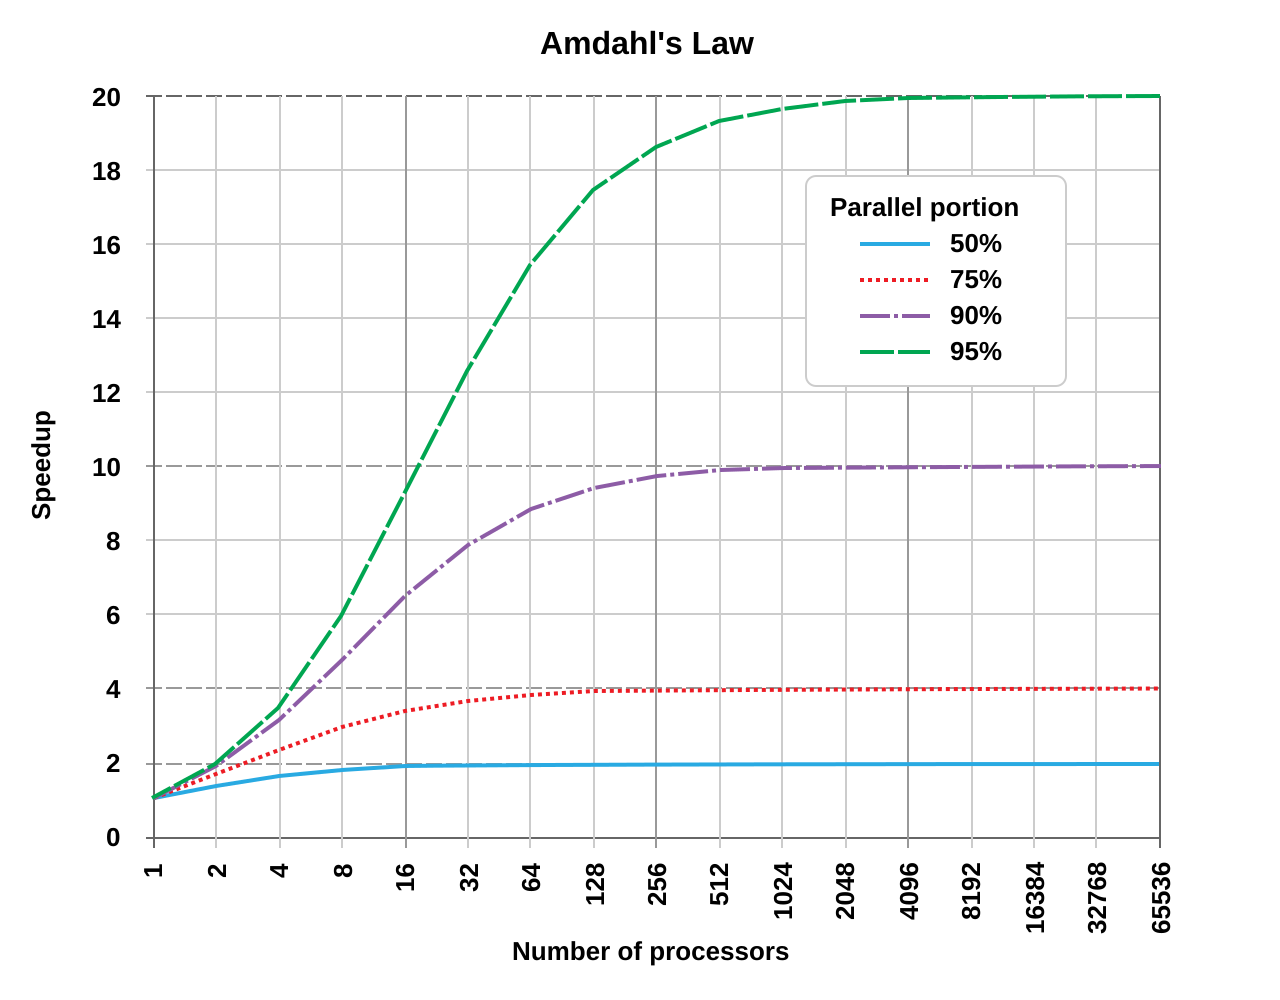
\includegraphics[width=0.3\textwidth]{./pics/amdahl.png}
\end{center}
\end{frame}

\begin{frame}[fragile]{Amdahl's law}
\framesubtitle{Examples}

\begin{itemize}
    \item Programmer enhances a part of the code that represents 10\% of the total execution time. This part starts to work \texttt{10 000} times faster. What is total speedup of a program?

    \item Problem could be split into two parts: A and B. A is serial, B is parallel. On single CPU, A takes 50 minutes, B takes 250 minutes. How many CPUs do you need to solve the problem in 100 minutes (achieve 3x speed-up)?

    \item Prepare an example where 10x speed-up could be achieved by using 100 CPUs only.
\end{itemize}

\pause

\begin{homeworkmail}{Task \taskAmdhal}{
    Provide answers and explanation for all three problems
}
\end{homeworkmail}

\end{frame}


\begin{frame}{Embarrassingly parallel problems}
\framesubtitle{Piece of advice}

Such problems usually quite interesting and practically-oriented.

They do \textbf{not} require non-trivial coordination so we will not cover them in this course.

In many domains, most of ''performance issues'' are (almost) embarrassingly parallel.

There are plenty of
\begin{itemize}
        \item easy-to-use
        \item straightforward
        \item safe
        \item stable
        \item performant
\end{itemize}
solutions to such problems. Just use them and get speed-up predicted by Amdahl's law.

If you go real concurrency, it will be \textbf{harder}.
\end{frame}

\begin{subsection}{Race condition}
\showTOCSub

\begin{frame}[fragile]{Race condition}
\framesubtitle{Example}

\begin{minted}{java}
public static void main(String... args) throws Exception {
    Thread t1 = new Thread(() -> { System.out.println("Thread A"); });
    Thread t2 = new Thread(() -> { System.out.println("Thread B"); });
    t1.start(); t2.start();
    t1.join(); t2.join();
}
\end{minted}

\pause

Execution 1: \texttt{Thread A Thread B}

Execution 2: \texttt{Thread B Thread A}

\end{frame}


\begin{frame}{Race condition}
\framesubtitle{Key idea}

\begin{itemize}
    \item Every single operation in program is OK (properly synchronized, atomic)
    \item Program as a whole suffers from non-deterministic behaviour
    \item The only reason to this is different speed of execution
\end{itemize}

\pause

\begin{homeworkmail}{Task \taskEmpire}{
    Open \url{https://deadlockempire.github.io}, pass all levels up to ''Confused counter'', inclusive.
}
\end{homeworkmail}
\end{frame}

\begin{frame}[t]{Race condition}
\framesubtitle{Conclusion}

Race condition
\begin{itemize}
    \item at least 2 threads involved
    \item behaviour of system depends on sequence of events (e.g. timings)
    \item leads to non-deterministic results
\end{itemize}

\pause 
Really \textbf{suspicious}
\begin{itemize}
    \item complicates analysis of algorithm (correctness, performance, resource utilization)
    \item may lead to rarely reproducible bugs
    \item may lead to random denial-of-service events
\end{itemize}

\end{frame}


\begin{frame}[t,noframenumbering]{Race condition}
\framesubtitle{Conclusion}

Race condition
\begin{itemize}
    \item at least 2 threads involved
    \item behaviour of system depends on sequence of events (e.g. timings)
    \item leads to non-deterministic results
\end{itemize}

Really \textbf{suspicious}
\pause

Not \textbf{necessarily} a problem
\begin{itemize}
    \item Server counts number of incoming requests.
    \item Search engine crawls page graph using several workers. Many pages visited several times, deduplication makes result consistent.
    \item Torrent client downloads several chunks of a file simultaneously.
\end{itemize}

\end{frame}

\begin{frame}[t,noframenumbering]{Race condition}
\framesubtitle{Conclusion}

Race condition
\begin{itemize}
    \item at least 2 threads involved
    \item behaviour of system depends on sequence of events (e.g. timings)
    \item leads to non-deterministic results
\end{itemize}

Really \textbf{suspicious}

Not \textbf{necessarily} a problem

\pause

Main headache of our course:
\begin{itemize}
 \item \textbf{Race condition may be a bug or intentional behaviour depending on programmer's intention}
\end{itemize}

In general, cannot be detected by static code analysis/dynamic instrumentation tool.
\end{frame}

\questiontime{Some tools detect race conditions in concurrent software. What is ''false positive'' detection of race condition?}

\begin{subsection}{Data race}
\showTOCSub

\begin{frame}[t,fragile]{Data race}
\framesubtitle{Example 1}

\begin{minted}{java}
static volatile int x = 0;
public static void main(String... args) throws Exception {
    Thread t = new Thread(() -> { x++; });
    t.start();
    System.out.println(x);
    t.join();
}
\end{minted}

\pause

Execution 1: \texttt{x = 0}

Execution 2: \texttt{x = 1}

\end{frame}

\begin{frame}[t,fragile]{Data race}
\framesubtitle{Example 2}

\begin{minted}{java}
static volatile int x = 0;
public static void main(String... args) throws Exception {
    Thread t = new Thread(() -> { x++; });
    t.start();
    x++;
    System.out.println(x);
    t.join();
}
\end{minted}

\pause

Execution 1: \texttt{x = 1}

Execution 2: \texttt{x = 2}
\end{frame}


\begin{frame}[t,fragile]{Data race}
\framesubtitle{Example 2.5}

\begin{minted}{java}
static volatile int x = 0;
public static void main(String... args) throws Exception {
    Thread t = new Thread(() -> { x++; });
    t.start();
    x++;
    t.join();
    System.out.println(x);
}
\end{minted}

\pause
Execution 1: \texttt{x = 2}

\pause 
Execution 2: \texttt{x = 1}

\pause

\texttt{x++ <=> int tmp = x;  tmp = tmp + 1; x = tmp} 

\end{frame}

\begin{frame}{Data race}
\framesubtitle{Key idea}

Actually, formal definition exists and is language-specific. More on this in next lectures.

Data race:
\begin{itemize}
    \item at least 2 threads
    \item at least one of threads is writing data
    \item operating on the same \textit{memory location} (Lecture~\cacheCoherencyNum)
    \item \textit{simultaneously} (Lecture~\foundationsNum)
    \item without \textit{proper synchronization} (Lecture~\langMMNum)
\end{itemize}

Any data race is race condition. Not every race condition is data race.

\end{frame}


\begin{frame}[fragile]{Data race}
\framesubtitle{Compound data example}

\begin{minted}{java}
static volatile ArrayList<String> list = new ArrayList<>();
public static void main(String... args) throws Exception {
    Thread t1 = new Thread(() -> { list.add("x"); });
    Thread t2 = new Thread(() -> { list.add("y"); });
    t1.start(); t2.start();
    t1.join(); t2.join();
    for (String s : list) {
      System.out.println(s);
    }
}
\end{minted}

\pause 

What is the size of \texttt{list}? \textbf{1} or \textbf{2}?

\pause

Data race may lead to \textbf{inconsistent} state even if every thread executed only ''valid'' operations.
\end{frame}

\begin{frame}[fragile]{Data race}
\framesubtitle{Word tearing}

\begin{minted}{java}
static volatile long data = 0;
public static void main(String... args) throws Exception {
    Thread t1 = new Thread(() -> { data = (1 << 0) + (1 << 33); });
    Thread t2 = new Thread(() -> { data = (2 << 0) + (2 << 33); });
    t1.start(); t2.start();
    System.out.println("data = " + data);
    t1.join(); t2.join();
}
\end{minted}

\pause

Is it possible to see \texttt{data == (1 << 0) + (2 << 33)}?

\pause
Depends on hardware, compiler and language. 

\end{frame}

\begin{frame}[fragile]{Data race}
\framesubtitle{Word tearing}

Java Language Specification\footnote{\url{https://docs.oracle.com/javase/specs/jls/se23/html/jls-17.html#jls-17.6}}

\begin{quote}
For the purposes of the Java programming language memory model, a single write to a non-volatile long or double value is treated as two separate writes: one to each 32-bit half. This can result in a situation where a thread sees the first 32 bits of a 64-bit value from one write, and the second 32 bits from another write.

Writes and reads of volatile long and double values are always atomic.

Writes to and reads of references are always atomic, regardless of whether they are implemented as 32-bit or 64-bit values.
\end{quote}

\pause

Data race may lead to \textbf{unexpected} state even if every thread executed only ''valid'' operations.
\end{frame}


\begin{frame}{Data race}
\framesubtitle{Benign data race}

%static boolean isPrime(int x) {
%    assert x > 1
%    for (int i = 2; i < x; i++) {
%      if (x % i == 0) return false
%    }
%    return true;
%}
%
%class EagerPrimeChecker {
%    final int number;
%    final boolean isPrime;
%
%    CachedPrimeChecker(int x) {
%      this.number = x;
%      this.isPrime = isPrime(x);
%    }
%
%    boolean isPrime() {        
%        return this.isPrime;
%    }
%}
%
%class LazyPrimeChecker {
%    final int number;
%    EagerPrimeChecker checker;
%
%    CachedPrimeChecker(int x) {
%      this.number = x;
%      this.checker = null;
%    }
%
%    boolean isPrime() {
%        if (this.checker == null) {
%            this.checker = new EagerPrimeChecker(this.number);
%        }
%        return this.checker.isPrime();
%    }    
%}
%
%main() {
%    final LazyPrimeChecker l = new LazyPrimeChecker(1_000_471);
%    t1 = new Thread() { -> println(l.isPrime()) } 
%    t2 = new Thread() { -> println(l.isPrime()) } 
%    t1.join()
%    t2.join();
%}

Data race that \textit{does not} affect correctness.

To be sure about this, you need to
\begin{itemize}
    \item understand all possible interleavings (Lecture~\extraBasicsNum) and memory ordering effects (Lecture~\cacheCoherencyNum)
    \item ensure particular language memory model allows such hacks (Lecture~\langMMNum)
    \item trust language compiler developers and language runtime engineers (Lecture~\designNum)
\end{itemize}

In our course \textbf{any} data race considered harmful.

\end{frame}


\begin{frame}{Data race}
\framesubtitle{Conclusion}

Data race is a specific variation of race condition 
\begin{itemize}
    \item concurrent and not properly synchronized    
    \item write access
    \item to shared data 
\end{itemize}

Always \textbf{problematic}
\begin{itemize}
    \item inconsistent shared state
    \item unexpected/impossible computation results
    \item forbidden by language implementation
\end{itemize}

Could be formalized and avoided
\begin{itemize}
    \item Strict coding policy (e.g. enforced by linter/compiler)
    \item Static analysis of source code
    \item Static analysis of execution traces
    \item Dynamic instrumenting race finders
\end{itemize}
\end{frame}

\questiontime{Some tools detect data races in concurrent software. Why do we still have systems with data races?}

\begin{subsection}{Visibility}
\showTOCSub


\begin{frame}{Visibility}
\framesubtitle{Introduction}

It is one of the most subtle notions in concurrency. 

\pause

For now, we should expect that 

\begin{itemize}
    \item compiler could aggressively reorder/eliminate field operations
    \item threads may see stale values, not the ''newest'' values written by other threads
\end{itemize}
\textbf{unless} there is ''synchronization point'' between two threads

\pause

\begin{itemize}
    \item \texttt{Thread.start}
    \item \texttt{Thread.join}
\end{itemize}

\end{frame}


\begin{frame}[fragile]{Visibility}
\framesubtitle{Incorrect: message passing via plain fields}

\begin{minted}{java}
static boolean jobDone = false;
public static void main(String... args) throws Exception {
    Thread t = new Thread(() -> { jobDone = true; });
    t.start();
    while (jobDone == false) { /* loop */ }
    t.join();
}
\end{minted}

\pause

May hang because:
\begin{itemize}
    \item compiler optimization: \texttt{if (!jobDone) while(true); }
    \item stale value, \texttt{jobDone} remains \texttt{false} in main thread forever
\end{itemize}
\end{frame}


\begin{subsection}{Deadlock}
\showTOCSub


\begin{frame}[t,fragile]{Blocking methods}
\framesubtitle{Wait-for graph}

Blocking method: execution of current thread is \textit{suspended} until some condition is met.

\begin{minted}{java}
Thread A = new Thread(() -> { 
    Thread B = new Thread(() -> { Thread.sleep(10_000); });
    Thread C = new Thread(() -> { B.join(); Thread.sleep(10_000); });
    B.start(); C.start(); B.join(); C.join()
}); A.start(); A.join();
\end{minted}

\pause

\begin{tikzpicture}[node distance=2cm,on grid,every state/.style={thick}]
  \node[state]  (main)              {$main$};
  \node[state]  (A) [right=of main] {$A$};
\end{tikzpicture}
\end{frame}


\begin{frame}[t,noframenumbering,fragile]{Blocking methods}
\framesubtitle{Wait-for graph}

Blocking method: execution of current thread is \textit{suspended} until some condition is met.

\begin{minted}{java}
Thread A = new Thread(() -> { 
    Thread B = new Thread(() -> { Thread.sleep(10_000); });
    Thread C = new Thread(() -> { B.join(); Thread.sleep(10_000); });
    B.start(); C.start(); B.join(); C.join()
}); A.start(); A.join();
\end{minted}

\begin{tikzpicture}[node distance=2cm,on grid,every state/.style={thick}]
  \node[state]  (main)              {$main$};
  \node[state]  (A) [right=of main] {$A$};
  \node[state]  (B) [right=of A]    {$B$};
  \node[state]  (C) [below=of B]    {$C$};
\end{tikzpicture}
\end{frame}

\begin{frame}[t,noframenumbering,fragile]{Blocking methods}
\framesubtitle{Wait-for graph}

Blocking method: execution of current thread is \textit{suspended} until some condition is met.

\begin{minted}{java}
Thread A = new Thread(() -> { 
    Thread B = new Thread(() -> { Thread.sleep(10_000); });
    Thread C = new Thread(() -> { B.join(); Thread.sleep(10_000); });
    B.start(); C.start(); B.join(); C.join()
}); A.start(); A.join();
\end{minted}

\begin{tikzpicture}[node distance=2cm,on grid,every state/.style={thick}]
  \node[state]  (main)              {$main$};
  \node[state]  (A) [right=of main] {$A$};
  \node[state]  (B) [right=of A]    {$B$};
  \node[state]  (C) [below=of B]    {$C$};

  \path[->] (main) edge  node   {} (A);
\end{tikzpicture}
\end{frame}

\begin{frame}[t,noframenumbering,fragile]{Blocking methods}
\framesubtitle{Wait-for graph}

Blocking method: execution of current thread is \textit{suspended} until some condition is met.

\begin{minted}{java}
Thread A = new Thread(() -> { 
    Thread B = new Thread(() -> { Thread.sleep(10_000); });
    Thread C = new Thread(() -> { B.join(); Thread.sleep(10_000); });
    B.start(); C.start(); B.join(); C.join()
}); A.start(); A.join();
\end{minted}

\begin{tikzpicture}[node distance=2cm,on grid,every state/.style={thick}]
  \node[state]  (main)              {$main$};
  \node[state]  (A) [right=of main] {$A$};
  \node[state]  (B) [right=of A]    {$B$};
  \node[state]  (C) [below=of B]    {$C$};

  \path[->] (main) edge  node   {} (A)                   
            (C)    edge  node   {} (B);
\end{tikzpicture}
\end{frame}

\begin{frame}[t,noframenumbering,fragile]{Blocking methods}
\framesubtitle{Wait-for graph}

Blocking method: execution of current thread is \textit{suspended} until some condition is met.

\begin{minted}{java}
Thread A = new Thread(() -> { 
    Thread B = new Thread(() -> { Thread.sleep(10_000); });
    Thread C = new Thread(() -> { B.join(); Thread.sleep(10_000); });
    B.start(); C.start(); B.join(); C.join()
}); A.start(); A.join();
\end{minted}

\begin{tikzpicture}[node distance=2cm,on grid,every state/.style={thick}]
  \node[state]  (main)              {$main$};
  \node[state]  (A) [right=of main] {$A$};
  \node[state]  (B) [right=of A]    {$B$};
  \node[state]  (C) [below=of B]    {$C$};

  \path[->] (main) edge  node   {} (A);
\end{tikzpicture}
\end{frame}











\begin{frame}[fragile]{Blocking methods}
\framesubtitle{Deadlock}

Deadlock -- cycle in wait-for graph.

Trivial single-threaded deadlock:
\pause
\begin{minted}{java}
    Thread.currentThread().join();
\end{minted}

\pause
Classic two-thread deadlock:

\begin{minted}{java}
    static volatile Runnable lambda = null; 
    public static void main(String... args) throws Exception {
        Thread A = new Thread(() -> { lambda.run(); });
        Thread B = new Thread(() -> { A.join();     }); 
        lambda = () -> { B.join(); };
        A.start(); B.start();
        A.join(); B.join();
    }
\end{minted}
\end{frame}


\begin{frame}[fragile]{Blocking methods}
\framesubtitle{Deadlock visualisation}

\begin{minted}{bash}
java Sample & 
PID="$!" && sleep 1
jstack -l $PID
\end{minted}

\pause

Output:
\begin{minted}{text}
"main" #1 prio=5 os_prio=0 cpu=38,96ms elapsed=1,25s tid=0x00007fdcc0017000 nid=0xcbc9a in Object.wait()  [0x00007fdcc538f000]
   java.lang.Thread.State: WAITING (on object monitor)
    at java.lang.Object.wait(java.base@14.0.1/Native Method)
    - waiting on <0x0000000095148930> (a java.lang.Thread)
    ...
    at Sample.main(Sample.java:10)
    ...
\end{minted}

\end{frame}


\begin{frame}{Blocking methods}
\framesubtitle{Deadlock detection}

\begin{itemize}
    \item If API has at least one blocking method -- extreme care required to avoid deadlocks
    \item If you do not know in which thread your code will be executed -- extreme care required to avoid deadlocks
    \item If you can not control execution (inheritance, virtual methods, function pointers) -- extreme care required to avoid deadlocks
    \item Design of any concurrent system should start with preparing tools for debugging and monitoring (observability API)
\end{itemize}

\pause

\begin{homeworkmail}{Task \taskJstack}{
    Run \texttt{jstack} on all deadlock samples from this lecture.
}
\end{homeworkmail}

\end{frame}

\questiontime{Object-oriented languages love to ''hide'' implementation details using abstractions (inheritance, virtual methods, function pointers, interfaces). How would I know that user of my library/module will not call blocking method and introduce deadlock in my system?}

\begin{subsection}{Priority inversion}
\showTOCSub


\begin{frame}[fragile]{Blocking methods}
\framesubtitle{Priority inversion}

\begin{minted}{java}
Thread A = new Thread(() -> { do1(); B = startThread(); do2(); B.join(); }); 
A.start();
doCriticalWork();
A.join();
\end{minted}

\texttt{main} waitsFor \texttt{A}, \texttt{A} waitsFor \texttt{B}.

Progress of \texttt{main} determined by progress of \texttt{B}.

''Soft'' version of deadlock (depends-on graph). 

\begin{itemize}
 \item Some Operation Systems \textbf{do} have special support to remedy priority inversion problems
 \item Many Virtual Machines, concurrent libraries, multi-threaded frameworks \textbf{do not}
\end{itemize}

\pause

If you launch rovers on Mars, be ready to debug them\footnote<2->{\url{https://www.cs.cornell.edu/courses/cs614/1999sp/papers/pathfinder.html}}.

\end{frame}


\begin{section}{Summary}

\begin{frame}{Summary}

\begin{itemize}
    \item We study agents with different speed that communicate with each other via shared memory
    \item Threads are parts of OS processes and are minimal unit of work for scheduler
    \item Tasks may be interrupted in pre-defined places or arbitrary allowing different levels of concurrency
    \item Independent tasks may be executed in parallel on different cores
    \item The perfect scenario: problem could be divided into many independent parts with almost zero coordination overheads
    \item Amdahl's law fundamentally limits possible speed-up of tasks with sequential parts
    \item Whenever you coordinate threads, you encounter race conditions, data races, visibility issues, deadlocks, priority inversion
\end{itemize}

\end{frame}

\begin{frame}{Summary: homework}

\begin{itemize}
    \item answer ''threads and exceptions'' question (Task~\taskExceptions)
    \item solve amdahl's law puzzles (Task~\taskAmdhal)
    \item \url{https://deadlockempire.github.io/} up to ''Confused Counter'' (Task~\taskEmpire)
    \item run \texttt{jstack} on deadlock samples (Task~\taskJstack)
\end{itemize}

% Small homework (2w)
% 
% interface MyFuture<T> {
%     T get();
% 
%     MyFuture<Y> andThen(Producer<Y> p);
% } 
% 
% public static MyFuture<T> computeOtherThread(Producer<T> p) {
% }
% 
% 
% Write documentation
% Transferring exceptions (*!! in seminar)
% Design tests
% O(n) andThen requires how many simultaneous threads?
% Future may hang, how to design API that is useful?
% prove no data races in implementation
% provide example with deadlocks for n-threads
\end{frame}

\end{document}
